\appendix

%-------------------------------------------------------------------------------
\section{Appendix}
\label{sec:appendix}
%-------------------------------------------------------------------------------

\subsection{Packet Processing Architectures} \label{subsec:rmt_drmt_overview}

\begin{figure}[h]
    \vspace{-1em}
     \centering
     \begin{subfigure}[h]{.42\textwidth}
         \centering
        \includegraphics[width=\textwidth]{figures/rmt}
        \caption{RMT architecture}
         \label{fig:rmt}
     \end{subfigure}
     \begin{subfigure}[h]{.42\textwidth}
         \centering
        \includegraphics[width=\textwidth]{figures/drmt}
         \caption{dRMT architecture}
         \label{fig:drmt}
     \end{subfigure}
     \caption{RMT vs dRMT}
    \label{fig:rmt_drmt}
\end{figure}

\vspace{-\baselineskip}
\vspace{-0.6em}

\subsection{RMT and dRMT Implementations} \label{subsec:rmt_drmt_implementations}
\vspace{-0.5em}

\begin{table}[h]
    \centering
    \small
    \setlength\extrarowheight{1.25pt}
    \setlength\tabcolsep{2.5pt}
    \begin{tabular}{lccc}
    \hline
      \thead[l]{Product} & \thead[c]{Architecture} & \thead[c]{Type} & \thead[c]{Sources} \\ 
        \hline
        Intel Tofino-2 & RMT & switch ASIC & \cite{tofino_rmt, tofino_slides, intel_tofino} \\
        Intel Mount Evans (E2000) & RMT & SmartNIC & \cite{e2000, intel_ipu} \\
        AMD Pensando DSC-100 & RMT & SmartNIC & \cite{amd_pensando, pensando_arch, pensando_p4} \\
        Fungible F1/S1 & RMT & SmartNIC & \cite{fungible} \\
        FlowBlaze & RMT & FPGA & \cite{flowblaze} \\
        FlexCore & dRMT & switch ASIC & \cite{flexcore} \\
        Nvidia BlueField-3 & dRMT & SmartNIC & \cite{nvidia_bluefield, nvidia_smartnic, nvidia_smartnic_2} \\
        \bottomrule
    \end{tabular}
    \caption{Summary of known implementations}
    \label{tab:implementations}
\end{table}

While we cannot verify all details in some cases, it is evident that TCAM, SRAM, parallelism, and programmability are present in the sources for the products listed in \cref{tab:implementations}.

\vspace{-0.5em}

\subsection{Updates, Deletions, and Insertions} \label{subsec:updates}

\subsubsection{\resail} \label{subsubsec:resailupdates}

Incremental updates, deletions, and insertions for \resail are efficient, following the same process as lookups but with modifications to the target entry. For prefixes of length $min\_bmp$ or greater, only two memory accesses are required~(bitmap and hash table). For prefixes shorter than $min\_bmp$, the operations are more costly because of prefix expansion. Update operations for prefixes longer than 24 bits are much simpler in \resail than in \sail because we have eliminated pivot pushing.

\vspace{-0.5em}

\subsubsection{\bsic} \label{subsubsec:bsicupdates}

For \bsic, incremental updates, deletions, and insertions are costly and complex due to inherent dependencies between binary search tree levels. A separate database with additional prefix information is needed for rebuilding data structures~\cite{dxr}. If fast update operations are important, \resail and \mashup are better choices.

\vspace{-0.5em}

\subsubsection{\mashup} \label{subsubsec:mashupupdates}
Incremental updates, deletions, and insertions for \mashup are nearly identical to lookups, except they modify the target entry. These are standard algorithms~\cite{network_algorithmics} for multibit tries that have been well studied. Maintaining a sorted TCAM table under these changes is non-trivial, but effective algorithms exist~\cite{tcam_updates}.

\vspace{-0.5em}

\subsection{Range Expansion and Optimizations} \label{subsec:bsic_details}

\vspace{-0.5em}

\begin{table}[h]
    \centering
    \small
    \setlength\extrarowheight{1.25pt}
    \setlength\tabcolsep{2.5pt}
    \begin{tabular}{|c|c|}
    \hline
    \thead[c]{Range} & \thead[c]{Next Hop} \\ 
    \hline
    0000 - 0011 & C \\
    0100 - 0100 & A \\
    0101 - 0111 & D \\
    1000 - 1001 & - \\
    1010 - 1010 & B \\
    1011 - 1011 & C \\
    1100 - 1111 & - \\
    \bottomrule
    \end{tabular}
    \caption{Range expansion for slice 1001 (\cref{tab:initial_lookup_table})}
    \label{tab:expansion_example}
\end{table}

\vspace{-\baselineskip}

\begin{figure}[h]
    \centering
    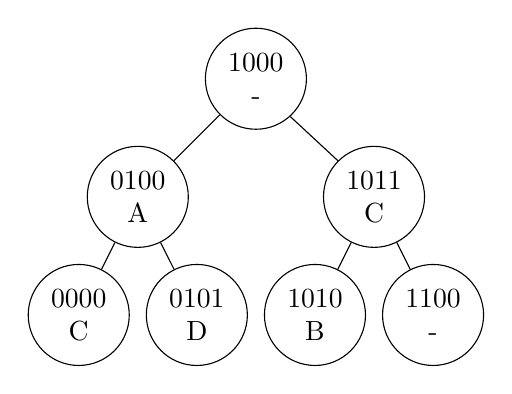
\begin{tikzpicture}[
      every node/.style = {minimum width = 2em, draw, circle, align=center},
      level/.style = {sibling distance = 30mm/#1}
      ]
      \node {1000\\-}
      child {node {0100\\A} 
            child {node {0000\\C}}
            child {node {0101\\D}}
            }
      child {node {1011\\C}
            child {node {1010\\B}}
            child {node {1100\\-}}
            };
    \end{tikzpicture}
    \caption{BST for slice 1001 (\cref{tab:initial_lookup_table})}
    \label{fig:tree_example}
\end{figure}

As in \dxr~\cite{dxr}, convert all the prefix substrings into ranges by generating their endpoint pairs. Use the endpoint pairs to create sorted, contiguous, and non-overlapping intervals that cover all possible bitstrings of the maximum length. Intervals that are added to complete the full range will "inherit" the next hop of the current lookup table entry's longest prefix match. This is necessary because it is possible for a destination address to be incorrectly directed by the initial lookup table to a BST that does not contain a legitimate match. Therefore, in the case of such a mistake, the search key will land in an interval containing the correct next hop. A simple example of range expansion for slice 1001 from \cref{tab:initial_lookup_table} is shown in \cref{tab:expansion_example}. Note that the intervals 1000-1001 and 1100-1111 were added to complete the full range. Since there are no valid longest prefix matches for slice 1001, its intervals are assigned a default value of -.

After the full range is created, merge neighboring intervals with the same next hop to reduce the number of nodes required. Discard the right endpoints as they can be inferred from the left ones. Use the remaining left endpoints to create the BST. \cref{fig:tree_example} shows a sample BST for slice 1001.

\vspace{-1em}

\subsection{Pseudocode} \label{subsec:pseudocode}

\begin{algorithm}[h]
    \SetKw{Break}{break}
    \SetKwInOut{KwIn}{Input}
    \SetKwInOut{KwOut}{Output}
    \KwIn{$addr$, IPv4 address}
    \KwIn{$min\_bmp$, smallest bitmap available}
    \KwOut{$hop$, next hop}
    $hop$ $\leftarrow$ $lookup\_table$.match($addr$)

    \If{$hop$ $\neq$ None}{\KwRet{$hop$}}
    
    \For{$i$ $\leftarrow$ 24 ; $i$ $\geq$ $min\_bmp$ ; $i$\texttt{{-}{-}}}{
        \If{$B_{i}$.match($addr$ $\gg$ (32-$i$)) \texttt{==} 1}
        {
            $key$ $\leftarrow$ ($addr$ $\gg$ (32-$i$)) $\ll$ (25-$i$)

            $key$ $\leftarrow$ $key$ + (1 $\ll$ (24-$i$))
            
            $hop$ $\leftarrow$ $hash\_table$.match($key$)

            \Break
        }
    }
    \KwRet{$hop$}
    \caption{\textbf{\resail Lookup} ($addr$, $min\_bmp$)} \label{alg:resail_lookup}
\end{algorithm}

\begin{algorithm}[h]
    \SetKw{Break}{break}
    \SetKwInOut{KwIn}{Input}
    \SetKwInOut{KwOut}{Output}
    \KwIn{$addr$, IPv4 or IPv6 address}
    \KwIn{$k$, initial slice size}
    \KwOut{$hop_{best}$, next hop}
    \SetKwFor{While}{while}{}{end while}%
    $level$ $\leftarrow$ 0

    $len$ $\leftarrow$ 32 if IPv4, 64 if IPv6
    
    $hop_{best}$,$index$ $\leftarrow$ $lookup\_table$.match($addr$ $\gg$ ($len-k$))

    \If{$hop_{best}$ $\neq$ None}{\KwRet{$hop_{best}$}}

    \While{$index$ $\neq$ None}{
        $hop$, $left$, $right$, $prefix$ $\leftarrow$ $bst_{level}$.match($index$)

        \If{$prefix$ \texttt{==} (($addr$ $\ll$ $k$) $\gg$ $k$)}{
            \KwRet{$hop$}
        }
        \ElseIf{$prefix$ < (($addr$ $\ll$ $k$) $\gg$ $k$)}{
            $index$ $\leftarrow$ $right$
            
            $hop_{best}$ $\leftarrow$ $hop$
        }
        \Else{
            $index$ $\leftarrow$ $left$
        }
        $level$ $\leftarrow$ $level$ + 1
    }
    \KwRet{$hop_{best}$}
    \caption{\textbf{\bsic Lookup} ($addr$, $k$)} \label{alg:bsic_lookup}
\end{algorithm}

\begin{algorithm}[h]
    \SetKw{Break}{break}
    \SetKwInOut{KwIn}{Input}
    \SetKwInOut{KwOut}{Output}
    \KwIn{$addr$, IPv4 or IPv6 address}
    \KwIn{$strides$, set of strides}
    \KwOut{$hop_{best}$, next hop}
    \SetKwFor{While}{while}{}{end while}%

    $hop_{best}$ $\leftarrow$ $default$
    
    $table$ $\leftarrow$ $root$

    $tag$ $\leftarrow$ None
    
    $index$ $\leftarrow$ 0

    $level$ $\leftarrow$ 0

    \While{$table$ $\neq$ None}{
        $key$ $\leftarrow$ $addr$[$index$:$index$+$strides$[$level$]]
        
        $hop$, $next\_table$, $tag$ $\leftarrow$ $table$.match($tag$, $key$)

        \If{$table$.hit()}{
            \If{$hop$ $\neq$ None}{
                $hop_{best}$ $\leftarrow$ $hop$
            }
            
            $index$ $\leftarrow$ $index$ + $strides$[$level$]
            
            $level$ $\leftarrow$ $level$ + 1

            $table$ $\leftarrow$ $next\_table$
        }
        \Else{
            \Break
        }
    }
    \KwRet{$hop_{best}$}
    \caption{\textbf{\mashup Lookup} ($addr$, $strides$)} \label{alg:mashup_lookup}
\end{algorithm}

% \vspace{-\baselineskip}

\subsection{Latency-memory trade-offs} \label{subsec:tradeoff}

A natural question is: {\em are there latency-memory trade-offs for CRAM algorithms that we can exploit to free up pipeline stages for other processing tasks?} Examining the basic \cram model, there appears to be a clear trade-off: reducing dependency steps at the expense of increased memory or computation can lead to lower latency. 

Unfortunately, on real platforms like Tofino-2, {\em steps} cannot be conflated with {\em stages} because, in RMT, stages provide a fixed amount of both memory and computation. Therefore, large lookup tables require multiple stages. While a latency-memory trade-off exists for {\em steps} versus memory in our three \cram algorithms, no corresponding trade-off exists for {\em stages} versus memory. Instead, there is an optimal number of stages, beyond which {\em both} memory and latency increase.

To see this, consider \cref{fig:latency_memory_tradeoff} for \bsic~(IPv6), in which the only tuning parameter is $k$---the width of the initial TCAM table. While a latency-memory curve exists, decreasing latency by increasing $k$ actually {\em increases} the number of stages required. As $k$ grows, the number of stages needed for the initial TCAM table rises significantly, outweighing the reduction in stages gained from decreasing BST depth. In contrast, the basic \cram model predicts reduced latency as $k$ increases. Unfortunately, this larger TCAM table requires more {\em stages} but not {\em steps}.

As shown in \cref{fig:latency_memory_tradeoff}, the optimal value of $k$ is 24, with both smaller and larger values yielding worse results. Thus, no trade-off exists between stages and memory. This is also the reason we use $k=24$ in our experiments for IPv6.

Similarly, with \mashup, the strides are the primary tuning parameter. Again, we did not find a useful memory-latency trade-off when considering stages. Finally, \resail consistently requires only two steps, with no latency-memory trade-off whatsoever in either the \cram or ideal RMT models.

While there is no useful latency-memory trade-off for a {\em fixed} database size in our three algorithms, an obvious trade-off emerges as the database size {\em increases}: the number of stages~(latency) must increase, at least to provide more memory. This is implicit in the linear trade-off curves shown in \cref{fig:ipv4_scaling} and \cref{fig:ipv6_scaling}. Notably, the y-axes in these figures represent SRAM pages. However, since more SRAM requires proportionally more stages, \cref{fig:ipv4_scaling} and \cref{fig:ipv6_scaling} can be rescaled to~(instead) depict stages versus database size, maintaining exactly the same curve shapes.

\begin{figure}[h]
    \centering
    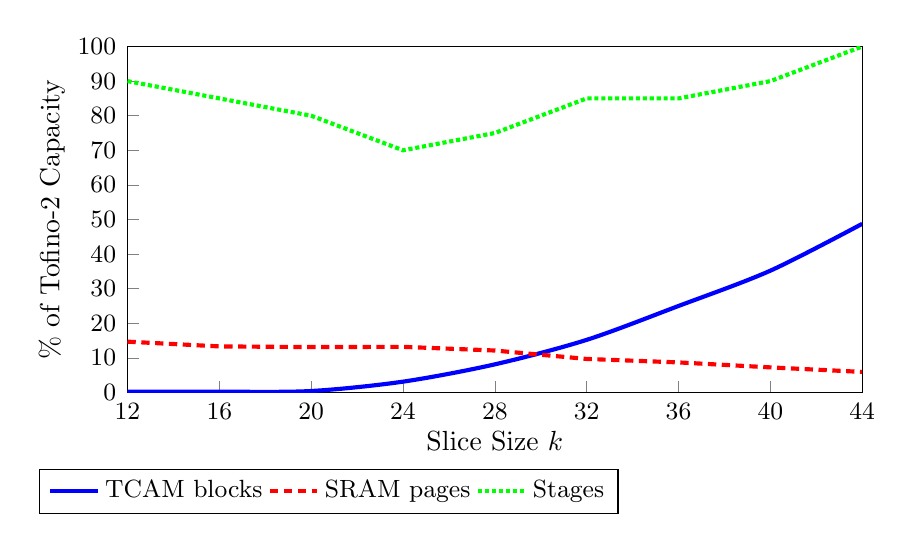
\begin{tikzpicture}
    \large
    \begin{axis}[
        xmin = 12, xmax = 44,
        ymin = 0, ymax = 100,
        xtick={12,16,...,44},
        ytick={0,10,...,100},
        width=\columnwidth*0.9,
        height=170pt,
        xticklabel={\ifdim\tick pt<10pt 0\fi\pgfmathprintnumber{\tick}},
        xticklabel style={rotate=0,font=\small},
        yticklabel style={rotate=0,font=\small},
        xlabel style={font=\normalsize,at={(axis description cs:.5,-.08)}},
        ylabel style={font=\normalsize,at={(axis description cs:-.07,.5)}},
        legend columns=3,
        legend style={at={(-0.12,-0.22)},anchor=north west,font=\small},
        xlabel=Slice Size $k$,
        ylabel=\% of Tofino-2 Capacity,
        tick pos=left
    ]
    \addplot[line width=1.5pt,mark=none,smooth,color=blue]
        coordinates{
            (12,0.2083333333)
            (16,0.2083333333)
            (20,0.4166666667)
            (24,3.125)
            (28,8.125)
            (32,15.20833333)
            (36,25)
            (40,35.20833333)
            (44,48.75)
        };
    \addlegendentry{TCAM blocks}
    \addplot[line width=1.5pt,mark=none,densely dashed,color=red]
        coordinates{
            (12,14.6875)
            (16,13.3125)
            (20,13.125)
            (24,13.1875)
            (28,12.125)
            (32,9.6875)
            (36,8.6875)
            (40,7.25)
            (44,5.9375)
        };
    \addlegendentry{SRAM pages}

    \addplot[line width=1.5pt,mark=none,densely dotted,color=green]
        coordinates{
            (12,90)
            (16,85)
            (20,80)
            (24,70)
            (28,75)
            (32,85)
            (36,85)
            (40,90)
            (44,100)
        };
    \addlegendentry{Stages}
    
    \end{axis}
    \end{tikzpicture}
    \caption{\bsic IPv6 latency-memory trade-off on an ideal RMT chip for AS131072 (Sep 2023)}
    \label{fig:latency_memory_tradeoff}
\end{figure}